\subsection{BERTopic}

Было произведено тематическое моделирование с использованием алгоритма $BERTopic$, который
обладает рядом преимуществ, указанных ранее.

В отличие от всех предыдущих методов, здесь нам потребуется другая предобратка текста: 
ранее мы удаляли из предложений редко встречаемые слова и стоп-слова (артикли, предлоги 
и так далее), сейчас же мы этого делать не будем. Делается этого по причине того, что
теперь для получения векторного представления предложений, вместо того, чтобы усреднять 
векторные представления всех входящих в него слов, это делается при помощи языковой модели 
$BERT$, которая была предобучена на огромном корпусе предложений. В обучаем корпусе не удалялись таких редкие слова и стоп-слова, так как при их удалении теряется некоторая часть
структуры предложения и также теперь векторные представления извлекаются у слов, учитывая их контекст внутри предложения. Поэтому теперь достаточно сделать всю ту очистку текста, 
которая была проведена ранее, за исключением удаления редких и стоп-слов.

В результате применения алгоритма получилось 1750 тем, из которых 13 состоят более чем
из 80 слов, для остальных тем ниже приведен рисунок распределения количества слов в темах:

\begin{figure}[H]
\centering
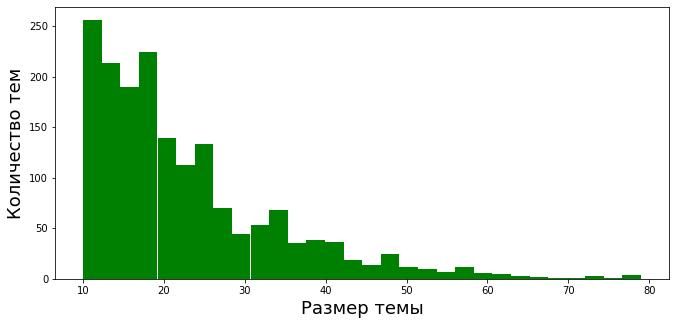
\includegraphics[scale=0.7]{pics/bert-size-distrib.png}
\caption{Гистограмма распределения размеров тем в результате работы алгоритма $BERTopic$
на наборе $Enron$}
\end{figure}


Данная модела сработало довольно неплохо, полученные темы получились интерпретируемы, ниже приведены некоторые из них:

\begin{table}[H]
\centering
\begin{tabular}{ | l | l | l | }
\hline
Номер кластера & Слова \\ \hline
261 & congrats, congratulations, exciting, promotions, jeff \\ \hline
327 & superstar, choate, wonderful, success, gifts, huge, 
\\ & nice, informative, kimberly, glad \\ \hline
1164 & drop, pick, damon, butch, dropping, picking,
\\ &  richie, rid, neal, kirby \\ \hline
394 & vpn, pending, applications, requested, id, 
\\ & natgas, jeffrey, phillip, application, jeff \\ \hline
\end{tabular}
\caption{Примеры полученных тем в результате работы алгоритма $BERTopic$ на наборе $Enron$}
\end{table}


Как и ранее, можно визуализировать темы в $2D$:

\begin{figure}[H]
\centering
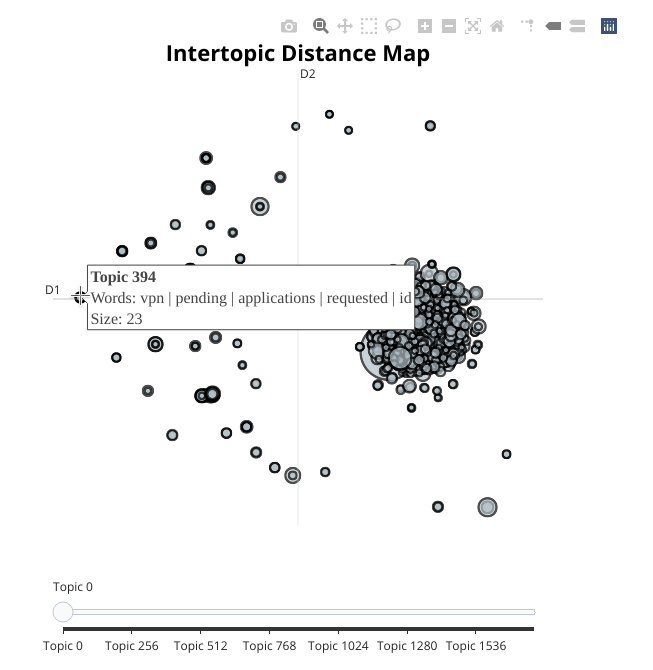
\includegraphics[scale=0.9]{pics/bert-2d-results.png}
\caption{Визуализации тем для модели $BERTopic$ на наборе $Enron$}
\end{figure}

В данном случае точки распределились не совсем равномерно, есть темы, расположенные далеко от
большого скопления точек, однако, как можно видеть на рисунке ниже, внутри этого скопления точки распределены равномерно: 

\begin{figure}[H]
\centering
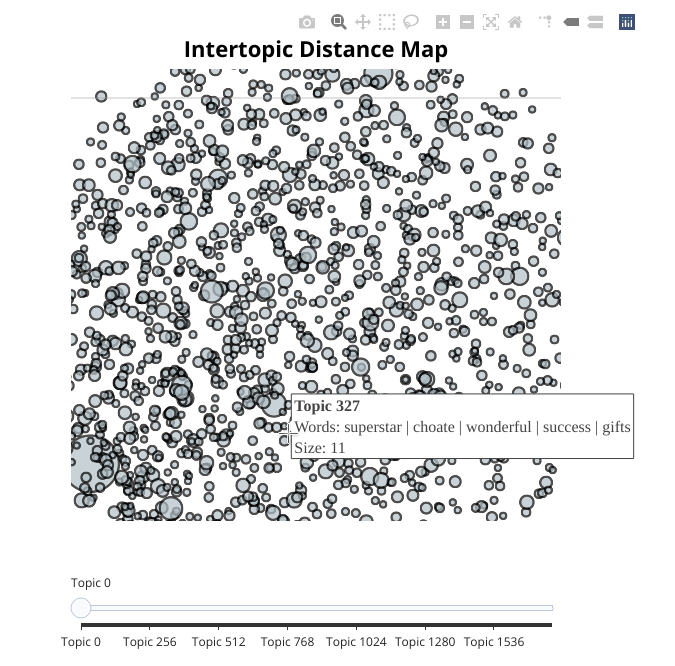
\includegraphics[scale=0.9]{pics/bert-circle.png}
\caption{Визуализация части скопления тем в $2D$ пространстве для модели $BERTopic$ на наборе $Enron$}
\end{figure}
